\chapter{The Main Screen}
\paragraph{Overview}
The Main Screen is the primary display screen. It is shown at power up, and is where Operation Mode (Hand or Automatic) is selected. It displays the Operator Message Centre which provides the Operator with current and relavent machine state information. There are aslo controls for \textit{Automatic \textbf{Cycle Start}} and \textit{Automatic \textbf{Cycle Stop}}, plus \textbf{\textit{Machine Full Stop}}. Finally, there are screen navigation keys provided for Operator access to other machine functions.
\begin{figure}
	\centering
	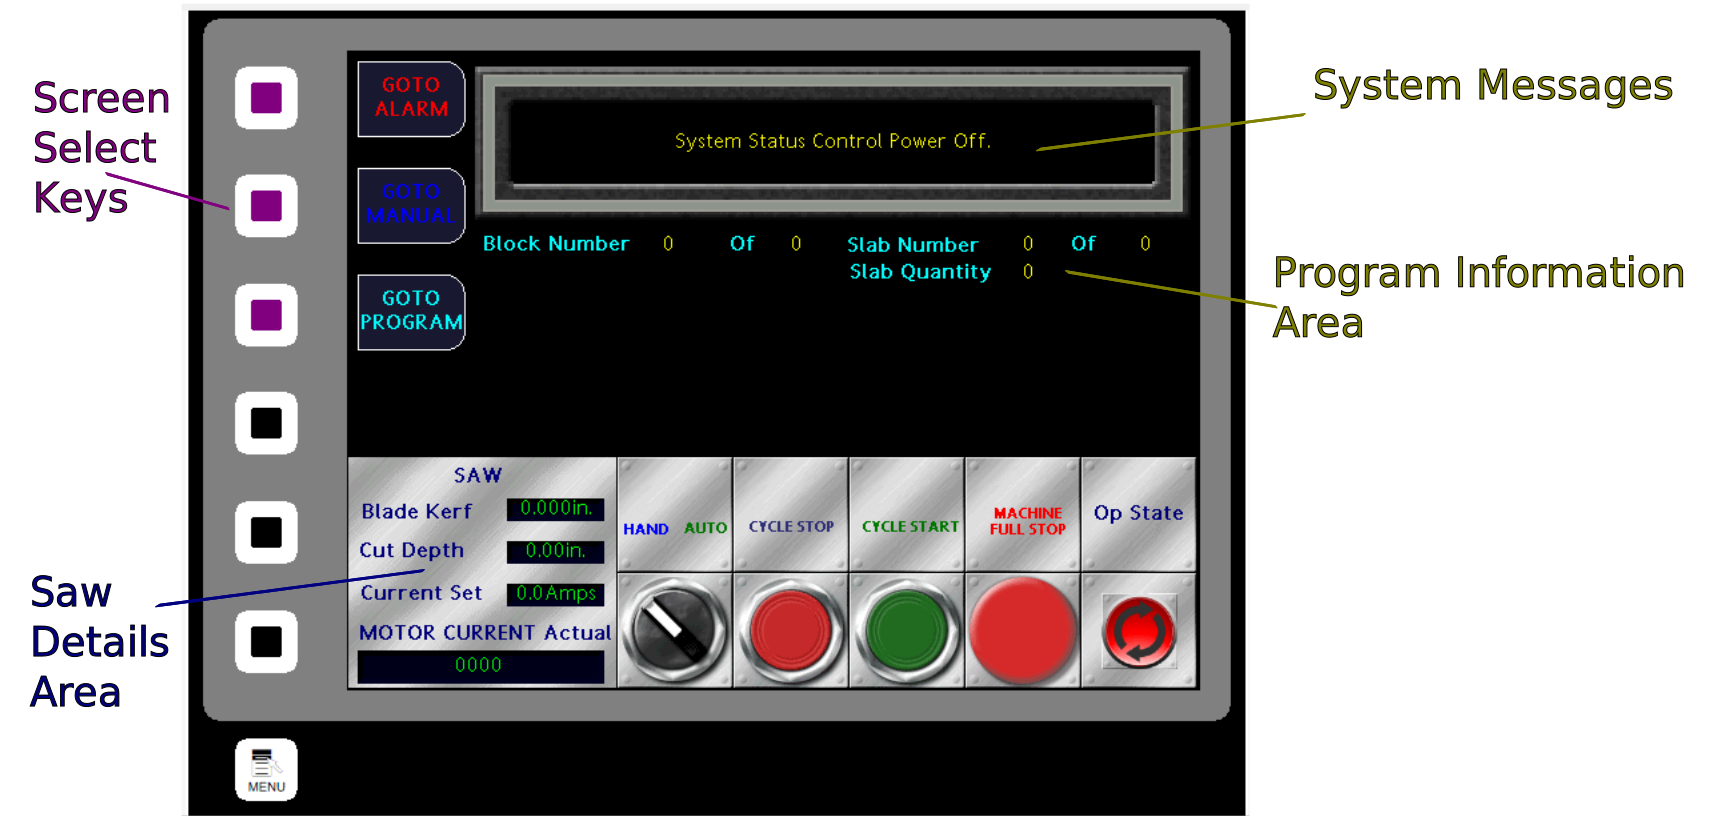
\includegraphics[width=0.5\linewidth]{screen-captures/main-screen}
	\caption{Main Screen}
	\label{fig:main-screen}
\end{figure}
\pagebreak
\paragraph{Main Screen Details}
Main Screen Details are divided into the general categories.
\begin{list}{-}{}
	\item \textbf{Screen Navigation}
	\item \textbf{Operator Message Centre}
	\item \textbf{Saw Information}
	\item \textbf{Program Details}
	\item \textbf{Operation Control}
\end{list}
\paragraph{Screen Navigation}Is performed by using the Programmable Keys (FKeys) located down the left hand side of the OI Terminal. For the Main Screen there are three screens accessible using the labeled FKey's, \textbf{Alarms}, \textbf{Manual}, and \textbf{Program}.
\\
\\
\\
\begin{minipage}{5cm}
	\begin{picture}(20,100)
	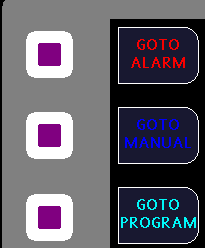
\includegraphics[width=.5\linewidth]{screen-captures/main-nav}
	\end{picture}
\end{minipage}\begin{minipage}[]{15cm}
	\textbf{GOTO ALARM} Navigate to Alarms Screen.
	\\
	\textbf{GOTO MANUAL} Navigate to Manual Screen.
	\\
	\textbf{GOTO PROGRAM} Navigate to Cut Program Screen.
\end{minipage}
\\
\paragraph*{\textbf{\LARGE \textcolor{blue}{i}}}
The Menu Key located on the terminal at the lower left below the FKey's, will return the Operator to the Main Screen, from all other screens.\\
\begin{minipage}{4cm}
	\begin{picture}(20,70)
	
\includegraphics[width=.5\linewidth]{screen-captures/menu}
	\end{picture}
\end{minipage}\begin{minipage}[]{11cm}
\paragraph{\textbf{\LARGE \textcolor{blue}{i}}} The Menu Key is pictured as it looks on the Terminal.
\end{minipage}
\pagebreak
\paragraph{Operator Message Centre}
Is the message display area located on the Main Screen near the Title. It is used to display information for the Operator during machine use. It doesn't display Alarms, that is done on the Alarms Screen, though it will indicate if an Alarm condition exists.
\\
\begin{picture}(0,60)

\includegraphics[width=.5\linewidth]{screen-captures/message-centre}
\end{picture}
\\
The \textbf{Operator Message Centre} shown above will display information messages for the Operator. If more than one message is active the display will scroll through all messages continuously.
\\
\paragraph{Saw Information}
Is an area where the Operator can see Saw information at a glance. \textbf{Saw Kerf}, \textbf{Cut Depth}, and \textbf{Current Set} are displayed along with the \textbf{Motor Current Actual}.
\\
\begin{picture}(0,165)
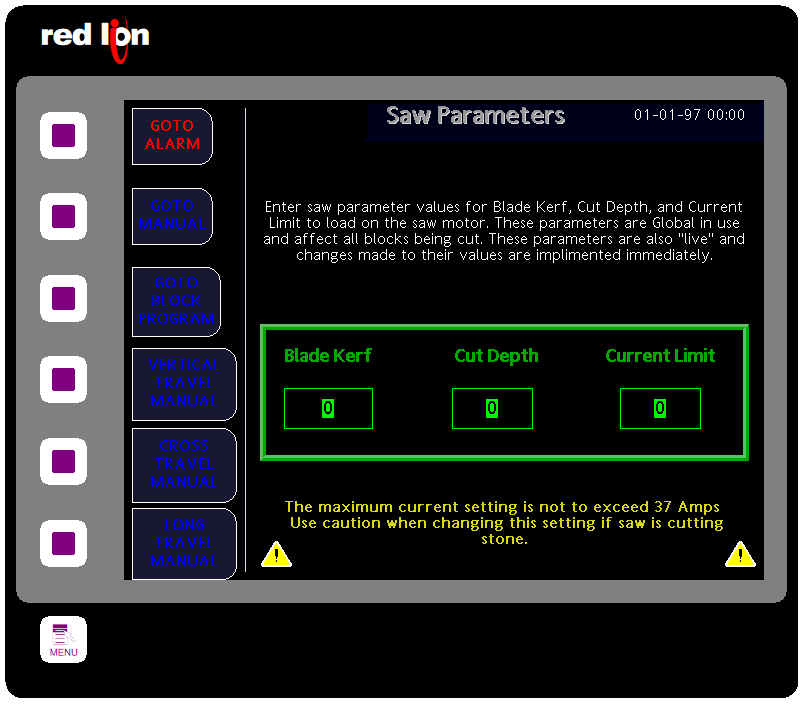
\includegraphics[width=.5\linewidth]{screen-captures/saw-info}
\end{picture}